
\section{Gatos y grandes números: cómo el muestreo modifica nuestra percepción}

\subsection{Introducción}

¿Alguna vez te has preguntado cuántos gatos hay realmente dentro de la UAM?

La pregunta parece sencilla, pero cuando varias personas comenzaron a discutir el tema aparecieron respuestas muy distintas. Algunos compañeros aseguraban que casi nunca veían gatos, mientras que otros afirmaban encontrarse varios todos los días, especialmente cerca de Villa Miau o en algunas zonas tranquilas del campus.

Incluso aparecieron comentarios como:

\begin{quote}
“en las tardes salen más”
\end{quote}

o bien:

\begin{quote}
“cuando hay mucho ruido desaparecen”.
\end{quote}

En ese momento surgió una idea interesante: transformar una observación cotidiana en un pequeño experimento estadístico.

La intención inicial no era únicamente contar gatos. En realidad, queríamos observar cómo cambian:

\begin{itemize}
\item las frecuencias observadas,
\item la media,
\item la varianza,
\item y las probabilidades empíricas
\end{itemize}

conforme aumenta el número de observaciones.

En otras palabras, buscábamos entender experimentalmente cómo el tamaño de muestra modifica nuestra percepción de un fenómeno.

\subsection{Objetivo}

Analizar cómo el tamaño de muestra modifica el comportamiento de estadísticos como la media y la varianza mediante un muestreo empírico de gatos dentro de la UAM Azcapotzalco.

\subsection{Diseño metodológico}

El experimento se desarrolló utilizando observación pasiva. Durante el estudio no se alimentó ni alteró el comportamiento de los animales con el objetivo de evitar introducir sesgos externos en las observaciones.

Las observaciones se realizaron en distintas zonas de la UAM Azcapotzalco, incluyendo:

\begin{itemize}
\item Villa Miau,
\item pasillos del edificio E,
\item jardineras,
\item estacionamientos,
\item plazas abiertas,
\item y zonas cercanas a biblioteca.
\end{itemize}

\subsection{Control experimental y regla antiduplicación}

Uno de los problemas más importantes del experimento fue evitar contar dos veces al mismo gato.

Para disminuir este problema se estableció una regla antiduplicación basada en:

\begin{itemize}
\item color del pelaje,
\item tamaño,
\item manchas,
\item color de ojos,
\item y dirección de movimiento.
\end{itemize}

Además, en algunos muestreos se realizaron observaciones simultáneas en distintas zonas con el objetivo de disminuir la probabilidad de doble conteo.

\subsection{Homogeneización del tiempo de observación}

Todos los equipos acordaron trabajar utilizando periodos homogéneos de:

\[
\boxed{2 \text{ minutos por observación}}
\]

De esta manera, cada muestra representa:

\begin{center}
\textit{el número de gatos observados durante un periodo fijo de dos minutos.}
\end{center}

\subsection{Duración y tamaño de muestra}

Es importante aclarar que los valores:

\[
n = 2,\; 5,\; 10,\; 15,\; 20
\]

no representan tiempo, sino el número total de observaciones realizadas.

Cada valor de \(n\) corresponde al número de veces que se repitió el proceso de observación de 2 minutos.

\subsection{Resultados experimentales: Equipo 1}

\subsubsection{Tablas de frecuencias}

\paragraph{\texorpdfstring{Resultados para \(n=2\)}{Resultados para n=2}}

\begin{table}[H]
\centering
\begin{tabular}{ccc}
\toprule
\(g\) & Frecuencia & PMF empírica \\
\midrule
0 & 0 & 0.00 \\
1 & 0 & 0.00 \\
2 & 1 & 0.50 \\
3 & 1 & 0.50 \\
4 & 0 & 0.00 \\
5 & 0 & 0.00 \\
\bottomrule
\end{tabular}
\caption{Distribución empírica para \(n=2\) (Equipo 1)}
\end{table}

Media: \(\bar{g}=2.50\) \quad Varianza: \(s^2=0.50\)

\paragraph{\texorpdfstring{Resultados para \(n=5\)}{Resultados para n=5}}

\begin{table}[H]
\centering
\begin{tabular}{ccc}
\toprule
\(g\) & Frecuencia & PMF empírica \\
\midrule
0 & 1 & 0.20 \\
1 & 0 & 0.00 \\
2 & 0 & 0.00 \\
3 & 1 & 0.20 \\
4 & 2 & 0.40 \\
5 & 1 & 0.20 \\
\bottomrule
\end{tabular}
\caption{Distribución empírica para \(n=5\) (Equipo 1)}
\end{table}

Media: \(\bar{g}=3.20\) \quad Varianza: \(s^2=3.70\)

\paragraph{\texorpdfstring{Resultados para \(n=10\)}{Resultados para n=10}}

\begin{table}[H]
\centering
\begin{tabular}{ccc}
\toprule
\(g\) & Frecuencia & PMF empírica \\
\midrule
0 & 1 & 0.10 \\
1 & 4 & 0.40 \\
2 & 1 & 0.10 \\
3 & 0 & 0.00 \\
4 & 1 & 0.10 \\
5 & 3 & 0.30 \\
\bottomrule
\end{tabular}
\caption{Distribución empírica para \(n=10\) (Equipo 1)}
\end{table}

Media: \(\bar{g}=2.60\) \quad Varianza: \(s^2=4.27\)

\paragraph{\texorpdfstring{Resultados para \(n=15\)}{Resultados para n=15}}

\begin{table}[H]
\centering
\begin{tabular}{ccc}
\toprule
\(g\) & Frecuencia & PMF empírica \\
\midrule
0 & 1 & 0.067 \\
1 & 2 & 0.133 \\
2 & 2 & 0.133 \\
3 & 3 & 0.200 \\
4 & 3 & 0.200 \\
5 & 4 & 0.267 \\
\bottomrule
\end{tabular}
\caption{Distribución empírica para \(n=15\) (Equipo 1)}
\end{table}

Media: \(\bar{g}=3.27\) \quad Varianza: \(s^2=2.92\)

\paragraph{\texorpdfstring{Resultados para \(n=20\)}{Resultados para n=20}}

\begin{table}[H]
\centering
\begin{tabular}{ccc}
\toprule
\(g\) & Frecuencia & PMF empírica \\
\midrule
0 & 3 & 0.15 \\
1 & 2 & 0.10 \\
2 & 2 & 0.10 \\
3 & 2 & 0.10 \\
4 & 3 & 0.15 \\
5 & 8 & 0.40 \\
\bottomrule
\end{tabular}
\caption{Distribución empírica para \(n=20\) (Equipo 1)}
\end{table}

Media: \(\bar{g}=3.35\) \quad Varianza: \(s^2=3.71\)

\subsection{Resultados experimentales: Equipo 2}

\subsubsection{Tablas de frecuencias}

\paragraph{\texorpdfstring{Resultados para \(n=2\)}{Resultados para n=2}}

\begin{table}[H]
\centering
\begin{tabular}{ccc}
\toprule
\(g\) & Frecuencia & PMF empírica \\
\midrule
0 & 0 & 0.00 \\
1 & 0 & 0.00 \\
2 & 0 & 0.00 \\
3 & 1 & 0.50 \\
4 & 0 & 0.00 \\
5 & 1 & 0.50 \\
\bottomrule
\end{tabular}
\caption{Distribución empírica para \(n=2\) (Equipo 2)}
\end{table}

Media: \(\bar{g}=4.00\) \quad Varianza: \(s^2=2.00\)

\paragraph{\texorpdfstring{Resultados para \(n=5\)}{Resultados para n=5}}

\begin{table}[H]
\centering
\begin{tabular}{ccc}
\toprule
\(g\) & Frecuencia & PMF empírica \\
\midrule
0 & 2 & 0.40 \\
1 & 1 & 0.20 \\
2 & 0 & 0.00 \\
3 & 2 & 0.40 \\
4 & 0 & 0.00 \\
5 & 0 & 0.00 \\
\bottomrule
\end{tabular}
\caption{Distribución empírica para \(n=5\) (Equipo 2)}
\end{table}

Media: \(\bar{g}=1.40\) \quad Varianza: \(s^2=2.30\)

\paragraph{\texorpdfstring{Resultados para \(n=10\)}{Resultados para n=10}}

\begin{table}[H]
\centering
\begin{tabular}{ccc}
\toprule
\(g\) & Frecuencia & PMF empírica \\
\midrule
0 & 4 & 0.40 \\
1 & 2 & 0.20 \\
2 & 2 & 0.20 \\
3 & 1 & 0.10 \\
4 & 1 & 0.10 \\
5 & 0 & 0.00 \\
\bottomrule
\end{tabular}
\caption{Distribución empírica para \(n=10\) (Equipo 2)}
\end{table}

Media: \(\bar{g}=1.40\) \quad Varianza: \(s^2=1.82\)

\paragraph{\texorpdfstring{Resultados para \(n=15\)}{Resultados para n=15}}

\begin{table}[H]
\centering
\begin{tabular}{ccc}
\toprule
\(g\) & Frecuencia & PMF empírica \\
\midrule
0 & 1 & 0.067 \\
1 & 3 & 0.200 \\
2 & 5 & 0.333 \\
3 & 2 & 0.133 \\
4 & 2 & 0.133 \\
5 & 2 & 0.133 \\
\bottomrule
\end{tabular}
\caption{Distribución empírica para \(n=15\) (Equipo 2)}
\end{table}

Media: \(\bar{g}=2.40\) \quad Varianza: \(s^2=2.26\)

\paragraph{\texorpdfstring{Resultados para \(n=20\)}{Resultados para n=20}}

\begin{table}[H]
\centering
\begin{tabular}{ccc}
\toprule
\(g\) & Frecuencia & PMF empírica \\
\midrule
0 & 3 & 0.15 \\
1 & 2 & 0.10 \\
2 & 3 & 0.15 \\
3 & 2 & 0.10 \\
4 & 2 & 0.10 \\
5 & 8 & 0.40 \\
\bottomrule
\end{tabular}
\caption{Distribución empírica para \(n=20\) (Equipo 2)}
\end{table}

Media: \(\bar{g}=3.10\) \quad Varianza: \(s^2=3.88\)

\subsection{Comparación entre equipos: convergencia de la media}

\begin{table}[H]
\centering
\begin{tabular}{lccccc}
\toprule
\textbf{Equipo} & \(\bar{g}_{2}\) & \(\bar{g}_{5}\) & \(\bar{g}_{10}\) & \(\bar{g}_{15}\) & \(\bar{g}_{20}\) \\
\midrule
Equipo 1 & 2.50 & 3.20 & 2.60 & 3.27 & 3.35 \\
Equipo 2 & 4.00 & 1.40 & 1.40 & 2.40 & 3.10 \\
\midrule
\textbf{Promedio} & 3.25 & 2.30 & 2.00 & 2.84 & 3.23 \\
\bottomrule
\end{tabular}
\caption{Convergencia de la media muestral por equipo. Ambos convergen hacia \(\approx 3.2\) gatos por observación.}
\end{table}

\subsubsection{Boxplots comparativos}

\begin{figure}[H]
\centering
\resizebox{0.98\linewidth}{!}{%
\begin{tikzpicture}
\begin{axis}[
    boxplot/draw direction=y,
    ylabel={Número de gatos observados},
    xlabel={Tamaño de muestra \(n\)},
    xtick={1,2,3,4,5},
    xticklabels={\(n=2\), \(n=5\), \(n=10\), \(n=15\), \(n=20\)},
    ymin=-0.5, ymax=5.5,
    ytick={0,1,2,3,4,5},
    width=14cm,
    height=8cm
]

\addplot+[boxplot prepared={lower whisker=2, lower quartile=2, median=2.5, upper quartile=3, upper whisker=3}] coordinates {};
\addplot+[boxplot prepared={lower whisker=0, lower quartile=3, median=4, upper quartile=5, upper whisker=5}] coordinates {};
\addplot+[boxplot prepared={lower whisker=0, lower quartile=0, median=1, upper quartile=5, upper whisker=5}] coordinates {};
\addplot+[boxplot prepared={lower whisker=0, lower quartile=1, median=3, upper quartile=5, upper whisker=5}] coordinates {};
\addplot+[boxplot prepared={lower whisker=0, lower quartile=0.75, median=3.5, upper quartile=5, upper whisker=5}] coordinates {};

\end{axis}
\end{tikzpicture}%
}
\caption{Diagramas de caja para el Equipo 1.}
\end{figure}

\subsection{El Teorema Central del Límite: aclaración fundamental}

Es común escuchar frases como:

\begin{center}
\textit{“cuando \(n\) es grande, los datos se distribuyen normal”.}
\end{center}

\textbf{Esto es incorrecto.}

El Teorema Central del Límite (TCL) no dice que la distribución de los datos originales se vuelva normal.  
Nuestros datos de gatos siguen siendo discretos (0,1,2,3,4,5) y con una forma que no es normal, incluso con \(n=20\).

\subsubsection{¿Qué dice realmente el TCL?}

El Teorema Central del Límite establece que:

\[
\boxed{\sqrt{n}\,\bigl(\bar{g} - \mu\bigr) \ \xrightarrow{d}\ \mathcal{N}(0,\sigma^2)}
\]

Es decir:

\begin{quote}
\textbf{La distribución de la media muestral \(\bar{g}\)} (no los datos individuales) se aproxima a una distribución normal conforme \(n\) aumenta.
\end{quote}

\subsubsection{Experimento mental con los gatos}

Imaginemos que repetimos muchas veces el experimento con \(n=20\):

\begin{itemize}
    \item Cada vez calculamos \(\bar{g}\) (el promedio de 20 observaciones).
    \item Esos promedios (no los gatos individuales) siguen una campana de Gauss.
\end{itemize}

Aunque un solo día veamos \(g = 0,5,2,1,3,0,5,\dots\) (discreto y no normal),  
el \textbf{promedio} de muchos días sí se comporta de manera normal.

\subsubsection{Visualización conceptual}

\begin{figure}[H]
\centering
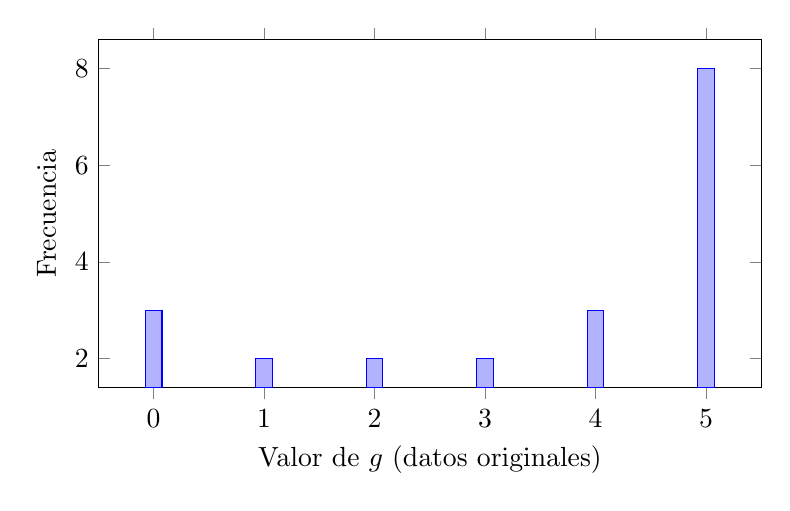
\begin{tikzpicture}
\begin{axis}[
    width=10cm,
    height=6cm,
    xlabel={Valor de \(g\) (datos originales)},
    ylabel={Frecuencia},
    ybar,
    bar width=6pt,
    xtick={0,1,2,3,4,5}
]
\addplot coordinates {(0,3) (1,2) (2,2) (3,2) (4,3) (5,8)};
\end{axis}
\end{tikzpicture}
\caption{Distribución de los datos originales (no es normal).}
\end{figure}

\begin{figure}[H]
\centering
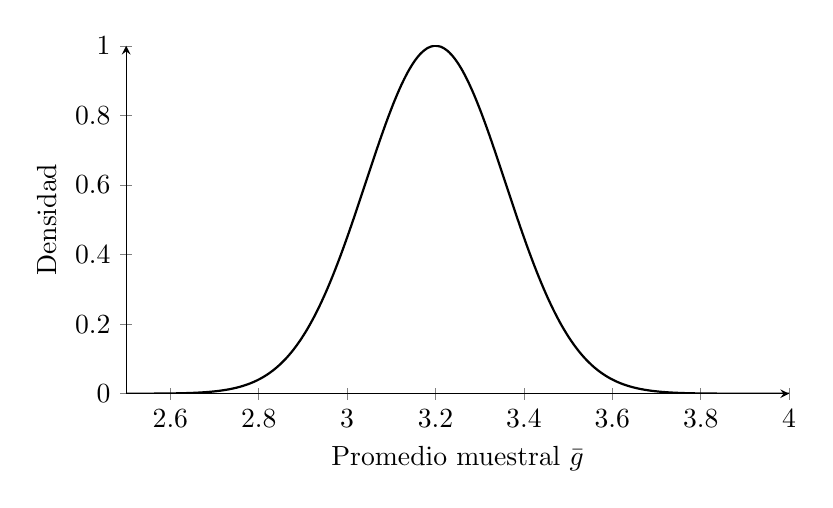
\begin{tikzpicture}
\begin{axis}[
    width=10cm,
    height=6cm,
    xlabel={Promedio muestral \(\bar{g}\)},
    ylabel={Densidad},
    domain=2.5:4.0,
    samples=100,
    axis lines=left
]
\addplot[thick, smooth] {exp(-20*(x-3.2)^2)};
\node at (axis cs:3.2,1.2) [anchor=south] {Aproximación normal};
\end{axis}
\end{tikzpicture}
\caption{Distribución de la \textbf{media muestral} \(\bar{g}\) (sí es normal).}
\end{figure}

\subsubsection{Consecuencia práctica}

\begin{quote}
\centering
\textit{El TCL nos permite usar la normal para hacer inferencias sobre la media,} \\
\textit{aunque los datos originales no sean normales.}
\end{quote}

Por eso podemos construir intervalos de confianza y pruebas de hipótesis sobre el número promedio de gatos en la UAM, incluso si cada observación individual es 0, 1, 2, 3, 4 o 5.

\subsection{Reflexión final}

Aunque el experimento parece sencillo, en realidad permite observar múltiples elementos fundamentales de estadística y probabilidad:

\begin{itemize}
\item construcción empírica de probabilidades,
\item estabilidad estadística,
\item variabilidad experimental,
\item convergencia,
\item Ley de los Grandes Números,
\item \textbf{Teorema Central del Límite}.
\end{itemize}

Más importante aún, muestra que conceptos como:

\[
\text{media},
\quad
\text{varianza},
\quad
\text{probabilidad},
\quad
\text{convergencia}
\]

no aparecen únicamente en ejercicios abstractos, sino también en fenómenos cotidianos aparentemente simples, como observar gatos dentro de una universidad.

\vspace{0.5cm}
\hrule
\vspace{0.2cm}
\begin{center}
\large
\textit{Con pocas observaciones → domina el azar} \\
\textit{Con muchas observaciones → aparece estabilidad} \\
\textit{El azar no desaparece… se organiza}
\end{center}

\begin{center}
\textbf{Eso es la Ley de los Grandes Números.}
\end{center}

\begin{center}
\textbf{Y el Teorema Central del Límite nos dice \textit{cómo} se organiza.}
\end{center}
